\chapter{Základné pojmy}

\label{kap:vychodiska} % id kapitoly pre prikaz ref

Táto kapitola slúži na oboznámenie čitateľa s pojmami a konceptmi používanými v ďalších častiach práce. Jednotlivé pojmy do potrebnej miery vysvetlíme a pri grafových reprezentáciách aj stručne naznačíme motiváciu za ich výberom, čo má pomôcť k lepšiemu pochopeniu ich potenciálnych prínosov.

\section{Logika prvého rádu}
\label{sec:fol}
Táto podkapitola vychádza najmä z prednášok a poznámok k predmetu Logika pre informatikov \cite{lpi}.

Logika prvého rádu je rodina formálnych jazykov, ktoré hovoria o objektoch a ich vlastnostiach. Symboly konkrétneho jazyka $\mathcal{L}$ logiky prvého rádu tvoria \textit{indivíduové premenné} (napr. $x$, $y$, $z$), \textit{logické symboly} ($\neg$, $\lor$, $\land$, $\rightarrow$, $\doteq$, $\exists$, $\forall$), \textit{pomocné symboly} (ľavá zátvorka, pravá zátvorka a čiarka) a \textit{mimologické symboly}, tie sa ďalej delia na \textit{indivíduové konštanty} (napr. Alice, FMFI), \textit{funkčné symboly} (napr. $f$, $g$) a \textit{predikátové symboly} (napr. $matka$, $spieva$). Indivíduové premenné, logické symboly a pomocné symboly sú rovnaké naprieč všetkými jazykmi logiky prvého rádu, čo však jednotlivé jazyky odlišuje sú použité mimologické symboly.

Predikátové symboly používame na označenie vlastností alebo vzťahov. V konkrétnom jazyku $\mathcal{L}$ vždy majú (spolu s funkčnými symbolmi) pevne zvolený počet argumentov, ktorý určuje ich \textit{arita}, niekedy označovaná horným indexom. Predikátové symboly s aritou 1 (unárne) zvyknú označovať nejakú vlastnosť alebo stav (napr. ${zviera}^1, {svieti}^1$), zatiaľ čo predikátové symboly s aritou 2 a viac ($n$-árne pre $n \geq 2$) opisujú určitý vzťah svojich argumentov (napr. ${stavia}^2$, ${ukazuje}^3$).

Ďalší zadefinujeme pojem \textit{term}. Každá indivíduová premenná a indivíduová konštanta jazyka $\mathcal{L}$ je term. Taktiež ak $f$ predstavuje funkčný symbol s aritou $n$ a $t_1, \dots, t_n$ sú termy, tak aj postupnosť symbolov $f(t_1, \dots, t_n)$ je term.

Ďalej každá postupnosť symbolov $t_1 \doteq t_2$, kde $t_1$ a $t_2$ sú termy predstavuje \textit{rovnostný atóm} a každá postupnosť symbolov $P(t_1, \dots, t_n)$, kde $P$ je predikátový symbol s aritou $n$ a $t_1, \dots, t_n$ sú termy predstavuje \textit{predikátový atóm}. Všetky rovnostné a predikátové atómy súhrnne nazývame \textit{atomickými formulami}.

Nakoniec množinu všetkých \textit{formúl} jazyka $\mathcal{L}$ definujeme takto: Každá atomická formula je zároveň aj formula. Ak $A$ je formula, tak aj postupnosť symbolov $\neg A$ je formula. Ak $A$ aj $B$ sú formuly, tak aj postupnosti symbolov $(A \land B)$, $(A \lor B)$, $(A \rightarrow B)$ sú formuly. A napokom ak $x$ je indivíduová premenná a $A$ je formula, tak aj postupnosti symbolov $\exists x A$ a $\forall x A$ sú formuly.


Prvým dôležitým pojmom týkajúcim sa sémantiky logiky prvého rádu je \textit{štruktúra}, ktorá sa vždy viaže na nejaký konkrétny jazyk. Označujeme ju dvojicou $\mathcal{M} = (D, i)$, kde $D$ predstavuje ľubovoľnú neprázdnu množinu (doména) a $i$ je zobrazenie (interpretačná funkcia). Úlohou interpretačnej funkcie je každej indivíduovej konštante priradiť prvok z $D$, každému funkčnému symbolu priradiť funkciu $f:D^n \rightarrow D$ a každému predikátovému symbolu priradiť podmnožinu množiny $D^n$, kde $n$ v oboch prípadoch označuje aritu daného symbolu. Štruktúry sú dôležitou súčasťou skúmania vlastností jazyka logiky prvého rádu, keďže poskytujú jeho presný matematický model.

Tiež zadefinujeme niektoré ďalšie pojmy. \textit{Ohodnotenie indivíduových premenných} je ľubovoľná funkcia $e: \mathcal{V}_\mathcal{L} \rightarrow D$, kde $\mathcal{V}_\mathcal{L}$ je množina indivíduových premenných. Potom \textit{hodnota termu} $t$ v štruktúre $\mathcal{M}$ pri ohodnotení premenných $e$ je prvok z $D$ označovaný $t^\mathcal{M}[e]$ definovaný nasledovne:
\[
    \begin{aligned}
        x^{\mathcal{M}}[e]                                & = e(x), \\
        a^{\mathcal{M}}[e]                                & = i(a), \\
        \left(f(t_1, \ldots, t_n)\right)^{\mathcal{M}}[e] & =
        i(f)\left(t_1^{\mathcal{M}}[e], \ldots, t_n^{\mathcal{M}}[e]\right),
    \end{aligned}
\]
pre všetky premenné $x$, všetky konštanty $a$, všetky funkčné symboly $f$ s aritou $n$ a všetky termy $t_1, \dots, t_n$.

Relácia $\mathcal{M} \models X[e]$ (čítame \textit{štruktúra }$\mathcal{M}$ \textit{spĺňa formulu} $X$ \textit{pri ohodnotení} $e$) je definovaná induktívne takto:
\[
    \begin{aligned}
        \mathcal{M} & \models t_1 = t_2 [e] \;\text{vtt}\; t_1^{\mathcal{M}}[e] = t_2^{\mathcal{M}}[e],                                      \\
        \mathcal{M} & \models P(t_1, \ldots, t_n)[e] \;\text{vtt}\; (t_1^{\mathcal{M}}[e], \ldots, t_n^{\mathcal{M}}[e]) \in i(P),           \\
        \mathcal{M} & \models \neg A [e] \;\text{vtt}\; \mathcal{M} \not\models A [e],                                                       \\
        \mathcal{M} & \models (A \land B)[e] \;\text{vtt}\; \mathcal{M} \models A[e] \;\text{a zároveň}\; \mathcal{M} \models B[e],          \\
        \mathcal{M} & \models (A \lor B)[e] \;\text{vtt}\; \mathcal{M} \models A[e] \;\text{alebo}\; \mathcal{M} \models B[e],               \\
        \mathcal{M} & \models (A \to B)[e] \;\text{vtt}\; \mathcal{M} \not\models A[e] \;\text{alebo}\; \mathcal{M} \models B[e],            \\
        \mathcal{M} & \models \exists x\, A[e] \;\text{vtt}\; \text{pre nejaký prvok } m \in D \text{ platí } \mathcal{M} \models A[e(x/m)], \\
        \mathcal{M} & \models \forall x\, A[e] \;\text{vtt}\; \text{pre každý prvok } m \in D \text{ platí } \mathcal{M} \models A[e(x/m)],
    \end{aligned}
\]
pre všetky premenné $x$, všetky formuly $A, B$, všetky termy $t_1, \dots, t_n$ a všetky predikátové symboly $P$ s aritou $n$.

\section{Grafové reprezentácie}
\label{sec:reprezentacie}

V tejto podkapitole sú uvedené typy grafov použité v tejto práci spolu s krátkym vysvetlením možností ich použitia. Niektoré definície vychádzajú z Grimaldiho učebnice diskrétnej matematiky \cite{grimaldi1985discrete}.

\subsection{Orientovaný graf}
Orientovaný graf $G$ je daný neprázdnou konečnou množinou vrcholov $V$ a množinou usporiadaných dvojíc $E \subseteq V \times V$, resp. hrán.
%pričom každá hrana $(x, y) \in E$ začína vo vrchole $x$ a končí vo vrchole $y$. 
V diagramoch sú vrcholy väčšinou znázornené ako kruhy, prípadne spolu s ich príslušným označením. Hrany sú zas vyobrazené pomocou šípok, ktorých smer určuje poradie vrcholov hrany (šípka vždy ukazuje na druhý vrchol v poradí). Majú mnohoraké využitie pri modelovaní vzťahov, ktoré vyžadujú zachovať nejaký smer, postupnosť úkonov alebo vyjadriť určitú hierarchiu. Príklad bežného diagramu jednoduchého orientovaného grafu možno vidieť na obrázku \ref{obr:dir_demo}, kde $V = \{1, 2, 3, 4\}$ a $E = \left\{(1, 2), (2, 3), (3, 1), (2, 4), (4, 2)\right\}$.

\begin{figure}
    \centerline{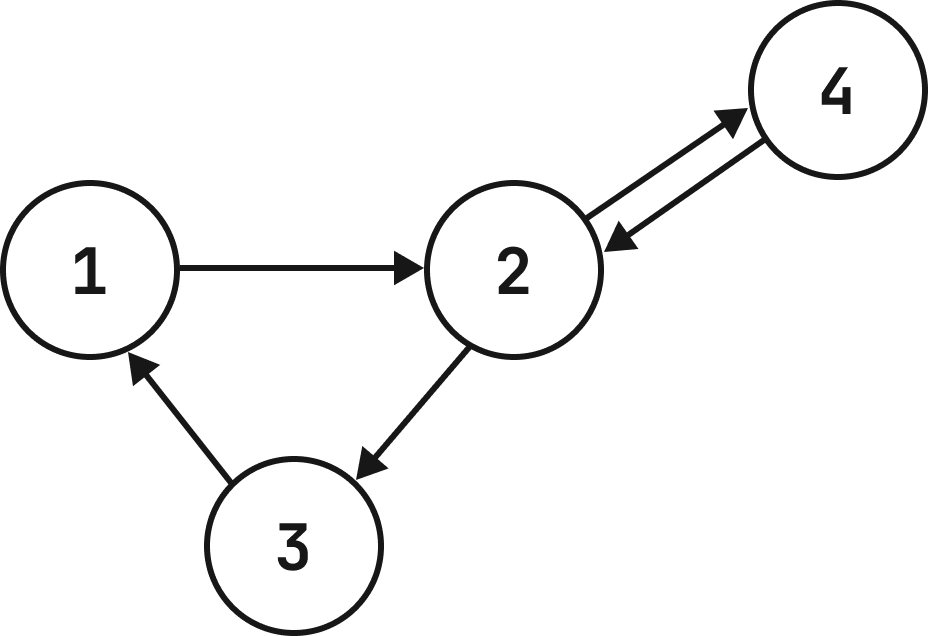
\includegraphics[width=0.4\textwidth]{images/directed-demo.png}}
    %popis obrazku
    \caption[Príklad vyobrazenia orientovaného grafu.]{Príklad vyobrazenia orientovaného grafu.}
    %id obrazku, pomocou ktoreho sa budeme na obrazok odvolavat
    \label{obr:dir_demo}
\end{figure}

\subsection{Hasseho diagram}
\label{sec:reprezentacie-hasse}

Pred opísaním Hasseho diagramu je najprv potrebné objasniť pojem čiastočného usporiadania, ktorý s ním veľmi úzko súvisí.

Podľa definície sa relácia $\leq$ na množine $A$ nazýva \textit{čiastočným usporiadaním}, ak je reflexívna, antisymetrická a tranzitívna. To znamená, že pre každé $x \in A$ musí platiť $x \leq x$ (prvok $x$ je v relácii so sebou samým - reflexívna relácia), pre každé $x,y \in A$ platí $(x \leq y \land y \leq x) \Rightarrow x = y$ (ak je prvok $x$ v relácii s prvkom $y$ a $y$ je v relácii s $x$, tak $x = y$ - antisymetrická relácia) a pre každé $x, y, z \in A$ platí $(x \leq y \land y \leq z) \Rightarrow x \leq z$ (ak je prvok $x$ v relácii s prvkom $y$ a $y$ je v relácii s prvkom $z$, tak aj $x$ je v relácii so $z$ - tranzitívna relácia). Intuitívnejšie si ale tento pojem možno predstaviť ako dvojice prvkov, z ktorých prvý vždy predchádza druhému. Zvyčajne sa čiastočné usporiadanie označuje aj ako dvojica $(A, \leq)$.

%rovnako ako v reálnom živote pri stavaní domu, kde je najprv potrebné položiť základy a až potom začať so stavbou strechy.

%Paralela s reálnym životom predstavuje napríklad natáčanie filmu, kde je najprv potrebné napísať scenár a až potom začať so strihom záberov.

%Teda ak by sme natáčanie filmu previedli do matematického sveta, označili by sme ho ako reláciu $R$ na $A$ a ľubovoľné úkony ako $x$ a $y$, kde vzťah $x R y$ značí, že $x$ a $y$ sú buď rovnaké, alebo $x$ sa musí uskutočniť pred začatím $y$.

Hasseho diagram slúži na prehľadnejšiu grafickú reprezentáciu čiastočných usporiadaní, keďže zachytáva iba bezprostredné vzťahy, bez zbytočného kreslenia hrán, ktoré intuitívne vyplývajú z jeho vlastností. Pri jeho tvorbe však treba dbať na dodržiavanie určitých pravidiel:
\begin{itemize}
    \item Každý prvok čiastočného usporiadania, teda prvok množiny $A$, je vrcholom v takomto grafe.
    \item Medzi ľubovoľnými prvkami $x, y \in A$ vytvárame hranu iba vtedy, keď $x \leq y$, $x \not = y$ a neexistuje taký prvok $z \in A$, rozdielny od $x$ a $y$, pre ktorý platí $x \leq z \leq y$.
    \item Ak je medzi prvkami $x, y \in A$ hrana a v usporiadaní platí $x \leq y$, potom vrchol reprezentujúci prvok $x$ kreslíme pod vrchol reprezentujúci prvok $y$.
\end{itemize}

Na obrázku \ref{obr:hasse_demo} možno vidieť príklad Hasseho diagramu pre čiastočné usporiadanie $(A, \mathcal{R})$, kde $A = \{2, 4, 5, 10, 20, 25\}$ a $x \, \mathcal{R} \, y$, ak $x$ delí $y$ bezozvyšku. Dobré je podotknúť, že aj prvky $2$ a $5$ sú v relácii s prvkom $20$, no hrany vyjadrujúce tento vzťah, ako bolo vyššie spomínané, nemusíme do diagramu explicitne zakresľovať.

\begin{figure}
    \centerline{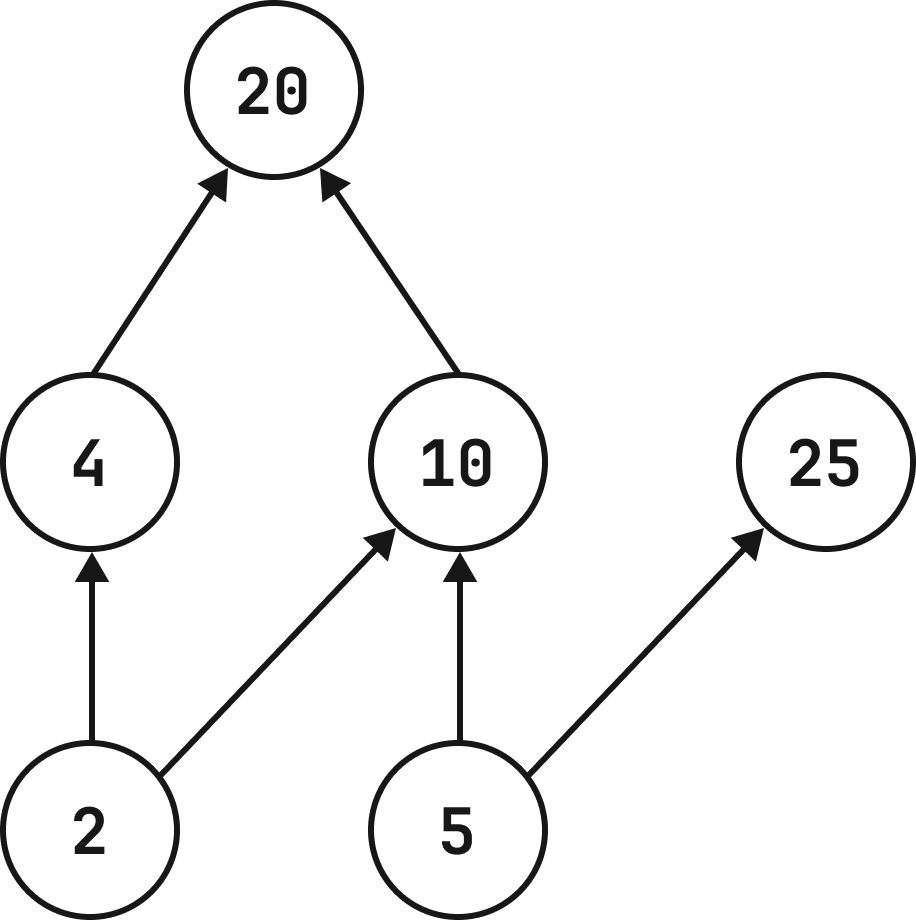
\includegraphics[width=0.4\textwidth]{images/hasse-demo.png}}
    %popis obrazku
    \caption[Príklad vyobrazenia Hasseho diagramu.]{Príklad vyobrazenia Hasseho diagramu.}
    %id obrazku, pomocou ktoreho sa budeme na obrazok odvolavat
    \label{obr:hasse_demo}
\end{figure}

%Tieto pravidlá umožňujú prehľadnejšie znázornenie jednotlivých vzťahov vyskytujúcich sa v usporiadaní.

\subsection{Bipartitný graf}
Bipartitný graf je taký graf $G$, ktorého vrcholy možno rozdeliť do dvoch disjunktných podmnožín $U$ a $V$ tak, že
$U \cap V = \emptyset$ a zároveň každá hrana spája jeden vrchol z $U$ s ďalším vrcholom z $V$ (alebo naopak). Vedia byť nápomocné pri hľadaní a skúmaní vzťahov (relácií a zobrazení) medzi entitami dvoch rôznych tried, ako napríklad medzi študentmi a učiteľmi, autormi a publikáciami alebo receptami a ingredienciami. Pri menšom množstve dát a vhodnom rozložení vrcholov umožňujú prehľadnú vizualizáciu prítomných vzťahov. Ukážku diagramu konkrétneho bipartitného grafu pre zobrazenie $f: \{1, 2, 3\} \rightarrow \{4, 5\}$, kde $f(1) = 4, f(2) = 5$ a $f(3) = 5$, so znázorneným rozdelením prvkov do množín $U$ a $V$ (v tomto prípade si možno predstaviť definičný obor a obor hodnôt zobrazenia) je vidieť na obrázku \ref{obr:bipartite_demo}.

\begin{figure}
    \centerline{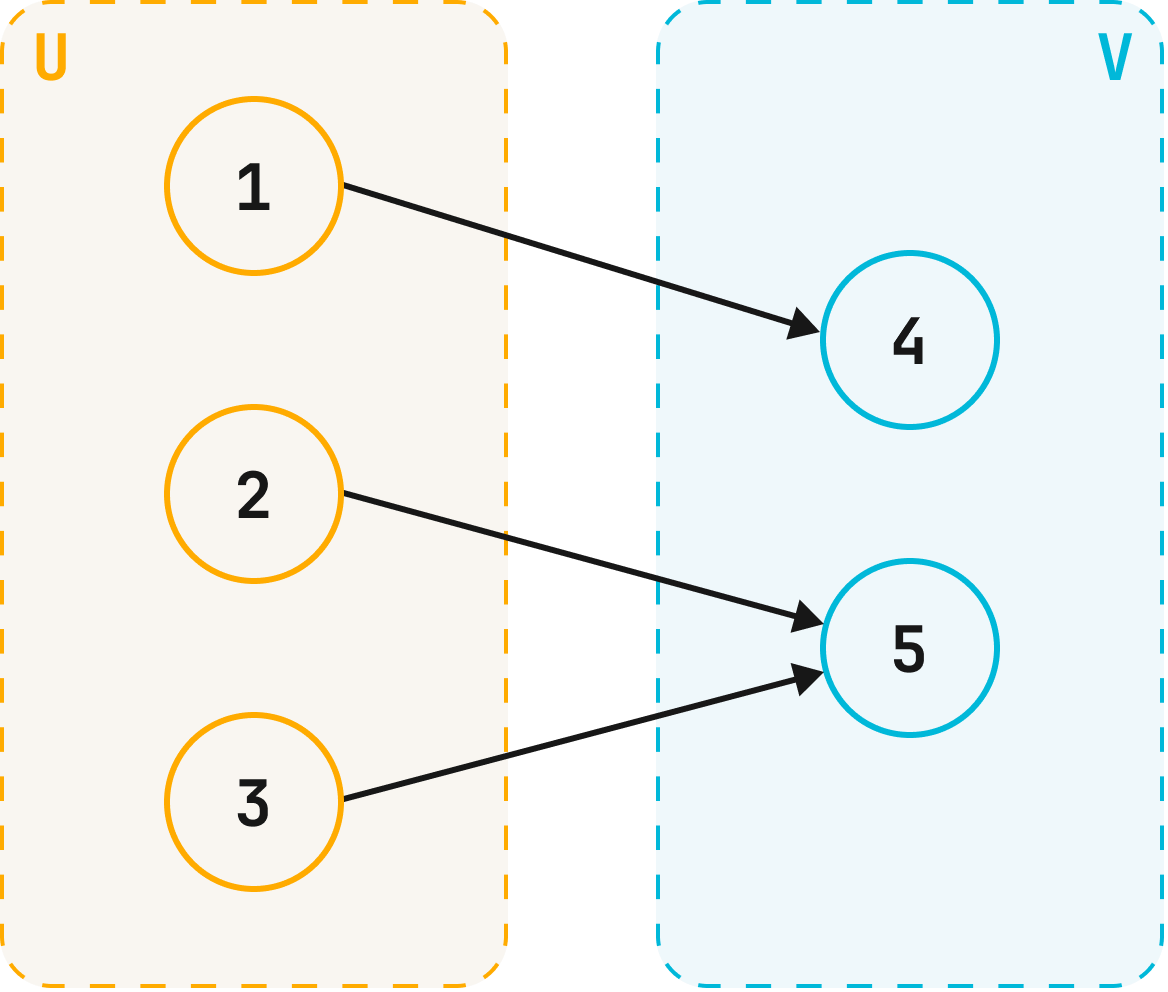
\includegraphics[width=0.5\textwidth]{images/bipartite-demo.png}}
    %popis obrazku
    \caption[Príklad vyobrazenia bipartitného grafu.]{Príklad vyobrazenia bipartitného grafu.}
    %id obrazku, pomocou ktoreho sa budeme na obrazok odvolavat
    \label{obr:bipartite_demo}
\end{figure}

\section{Použité technológie}
\label{sec:technologie}

V tejto podkapitole sú uvedené kľúčové technológie použité pri implementácii.

\subsection{React}
React \cite{react} je v súčasnosti jedna z najpopulárnejších JavaScriptových knižníc na tvorbu responzívnych webových aplikácií.

Základnú stavebnú jednotku tvorí komponent, čo je JavaScriptová funkcia, ktorá produkuje určitý strom elementov jazyka HTML, ďalej označovaný ako markup. Každý takýto komponent potom predstavuje konkrétnu časť používateľského rozhrania s vlastnou funkcionalitou a vzhľadom.

Vo väčšine prípadov sa markup komponentov zapisuje vo forme JavaScript XML (JSX), čo je syntaktické rozšírenie jazyka JavaScript. JSX je veľmi podobný značkovaciemu jazyku HTML, no umožňuje používanie vlastných značiek, ako aj jednoduchšiu manipuláciu s dynamickým obsahom. Toto je pre React kľúčové, keďže je tým umožnené skladať viaceré reaktívne komponenty do určitej hierarchie, ktorá reprezentuje celú aplikáciu.

%Ďalšou dôležitou súčasťou React-u je tzv. \verb'state', alebo stav komponentu. Zmena tohoto stavu spôsobuje, že sa celý komponent spracuje nanovo, už ale s aktuálnou hodnotou stavu. Na jeho základnú reprezentáciu sa používa špeciálna funkcia \verb|useState()|. Tejto funkcii môžeme dať ako parameter počiatočnú hodnotu stavu, ona nám vráti dvojicu aktuálnej hodnoty stavu, ako aj funkciu na zmenu tohoto stavu. Táto a s ňou aj iné funkcie poskytnuté React-om predstavujú tzv. \verb'hook', čo je funkcia ktorou sa vieme napojiť na niektoré vnútorné mechanizmy nášho komponentu.



\subsection{TypeScript}
TypeScript \cite{typescript} je programovací jazyk s podporou pre statické typy s konfigurovateľnou mierou typovej kontroly. Funguje iba ako syntaktické rozšírenie JavaScriptu, ktoré sa pri kompilácii naspäť zmení na čistý JavaScript. Práve táto vlastnosť zapríčiňuje jeho širokú kompatibilitu s už existujúcim ekosystémom.

Statické typovanie pomáha odhaľovať chyby už v skorých fázach vývoja, zlepšuje čitateľnosť aj udržateľnosť kódu a vývojárskym prostrediam umožňuje integráciu bohatšej funkcionality, ako napríklad pokročilejšie automatické dopĺňanie na základe kontextu alebo vyhľadávanie definícií. Svojimi prínosmi teda dokáže priamo aj nepriamo uľahčiť a spríjemniť prácu samotného programátora.

Jazyk poskytuje možnosť definovať rozhrania pomocou kľúčového slova \verb|interface|, ktoré upresňujú zamýšľaný tvar objektov. Kľúčové slovo \verb|type| zas umožňuje vytváranie typových aliasov, či už primitívnych alebo komplexných typov. Okrem samotných typov podporuje typovú inferenciu, čo pomáha s prehľadnosťou programu, keďže často nie je potrebné tvar objektu definovať manuálne.

\subsection{React Flow}
React Flow \cite{reactflow} je populárna knižnica na tvorbu grafových editorov, ktorá je súčasťou väčšieho projektu xyflow \cite{xyflow}. Zatiaľ čo React Flow je určený pre React, xyflow ponúka plnú kompatibilitu aj s niektorými inými podobnými knižnicami. Jej veľkou výhodou je široká škála možností prispôsobenia jednotlivých aspektov grafu, ako aj ich jednoduchá implementácia.

Každý vrchol predstavujú jeho atribúty a príslušný React komponent. Atribúty musia byť minimálne tvorené pozíciou a unikátnym identifikátorom. Ďalej však môžeme pridávať vlastné atribúty, ako aj komponenty, ktoré sa dajú prispôsobiť špecifickým potrebám našej aplikácie. Na veľmi podobnom princípe sa dajú konfigurovať aj hrany grafu, tie sú tiež tvorené komponentmi a spolu s vrcholmi tvoria základnú štruktúru každého grafu.

Knižnica tiež poskytuje niektorú rozšírenú funkcionalitu, akou je napríklad centrovanie grafov, uloženie a obnovenie stavu grafu alebo
konfigurovateľný panel s nástrojmi.

\subsection{Redux}
Redux \cite{redux} je knižnica na správu stavu JavaScriptových aplikácií, často používaná spolu s knižnicou React na zjednodušenie tvorby komplexných používateľských rozhraní. Stav aplikácie je reprezentovaný iba ako obyčajný objekt, ktorý predstavuje centrálne miesto pre ukladanie a čítanie dát, čím výrazne uľahčuje ich zdieľanie naprieč komponentmi.

Stav v Reduxe nie je možné meniť priamo. Namiesto toho sa zmeny vykonávajú pomocou akcií a reducerov. Akcie sú objekty popisujúce konkrétnu udalosť v aplikácii. V prípade potreby môžu obsahovať aj doplňujúce údaje (payload). Tieto akcie ďalej spracúvajú reducery. To sú funkcie, ktoré na základe aktuálneho stavu a prijatej akcie určia nový stav aplikácie. Pre ich správne fungovanie je dôležité dbať na to, aby reducer pre rovnaký stav a rovnakú akciu vždy vrátil rovnaký výsledok, nemali by sa preto používať napríklad na generovanie náhodných hodnôt. Aplikácia môže obsahovať viacero reducerov, čo umožňuje rozdeliť logiku na menšie, nezávislé časti.

Na získavanie konkrétnych dát zo stavu sa používajú selektory. Ide o funkcie, ktoré na základe súčasného globálneho stavu vyberajú alebo odvodzujú potrebné údaje, čím zjednodušujú a sprehľadňujú prácu s dátami.

